\subsection{kc3ddip:Dip}
The class \textbf{Dip} represents a thru-hole DIL package. The general
case parameters are set by invoking the member function \textbf{setParams(params)} where
params is a DipParams object with the following members:

\begin{itemize}
\item\textbf{A1} height from top of PCB to bottom of case\\
\item\textbf{A2} height of case\\
\item\textbf{L} depth of pin from top of PCB\\
\item\textbf{e} pin pitch\\
\item\textbf{E} row spacing\\
\item\textbf{E1} case width\\
\item\textbf{B1} wide portion of pin\\
\item\textbf{b} narrow portion of pin\\
\item\textbf{c} pin thickness\\
\item\textbf{NW} notch width (nominal 0.06 inch)\\
\item\textbf{ND} notch depth (nominal 0.012 inch)\\
\item\textbf{NL} notch length (nominal 0.07 inch, must be $>\textrm{ND}$)\\
\item\textbf{casebev} bevel on case (nominal 0.005 inch)\\
\item\textbf{pinbev} bevel on pin (nominally $\textrm(c)/10$)\\
\item\textbf{MID} height of middle case portion where pin attaches (nominally $1.4*\textrm{c}$);
    set to a negative number to default to the nominal value\\
\item\textbf{DW} extra length on case (nominal $2*(\textrm{c}/3 + \textrm{B}1/2)$);
    set to a negative number to default to the nominal value\\
\item\textbf{S} deviation of unbeveled top and bottom edged from mid section (taper);
    set to a negative number to default to the nominal value (5 degree taper)\\
\item\textbf{scale} scale factor to apply to final output\\
\item\textbf{rotation} rotation (radians) along Z axis for final output\\
\end{itemize}


The remaining Dip class member functions are as follows:

\textbf{setPins(npins)} sets the nominal number of pins to npins; npins must
be $\ge4$ and must be a multiple of 2. The nominal number of pins is used in
calculating the total length of the package. The nominal number is the maximum
number of pins which can be attached to the package; the pins which are
actually rendered are controlled via the \textbf{setPin()} function.
Return values are 0 for success and -1 for failure.

\textbf{setPin(pin, on)} selects whether a specific pin should be rendered or
not. By default all pins are rendered unless this routine is invoked to suppress
a pin. Return values are 0 for success and -1 for failure.

\textbf{setPinColor(filename)} and \textbf{setCaseColor(filename)} load
a material appearance file for the pin and case. These functions return 0
for success and -1 for failure.

\textbf{create(filename)} calculates the model features and writes the
result to the specified filename. Return values are 0 for success and -1 for failure.

The example below creates two DIL-12 packages; one has a complete set of pins while
the other only has the 2 pins in each corner. This demonstrates how the software
can be used to generate typical DIP models as well as specialised models, such as
packaged reed relays, which may be missing pins.

\begin{verbatim}
import kc3ddip
from kc3ddip import *

# the parameters are initialized to suit 0.3" pitch
p = DipParams()


dil = Dip()
dil.setParams(p)
dil.setPins(12)
# we need to specify colors
dil.setPinColor("../colors/tin.mat")
dil.setCaseColor("../colors/ceram_gry.mat")

# write out the normal DIP
dil.create("DIL_12_plain.wrl")

# suppress pins; note that pins are numbered from 1..N
dil.setPin(3, False)
dil.setPin(4, False)
dil.setPin(9, False)
dil.setPin(10, False)

# write out the special DIP
dil.create("DIL_12_special.wrl")
\end{verbatim}

\begin{figure}
\label{fig:k3ddipn}
\centering
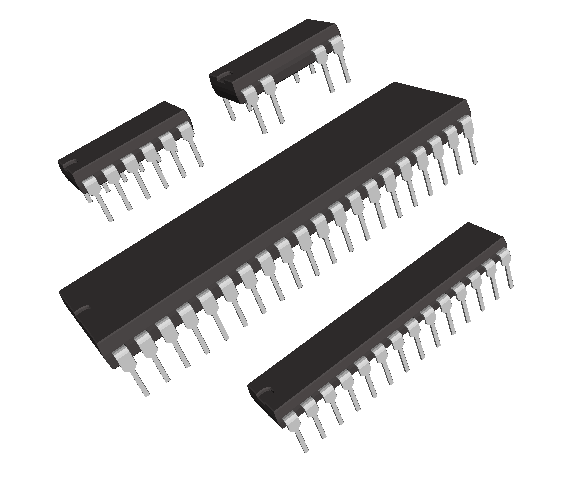
\includegraphics[width = 0.5\textwidth]{img/k3ddipn.png}
\caption{DIL packages produced from the model. From left and top
the models are 12-pin DIL with 0.3 inch rows, 12-pin DIL
with 0.3 inch rows and 4 pins removed, 40-pin DIL with 0.6 inch
rows, and 28-pin DIL with 0.3 inch rows.}
\end{figure}


